\subsection{张量代数的函子性质}

命题2. 设A是一个交换环，M和N是两个A-模，且

\[
u: \mathbf {M} \rightarrow \mathbf {N}
\]

为一个A-线性映射。存在唯一一个A-代数同态

\[
u ^ {\prime}: \mathsf {T} (\mathbf {M}) \rightarrow \mathsf {T} (\mathbf {N})
\]

使得图表

\pandocbounded{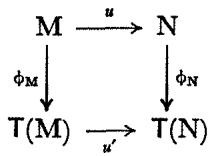
\includegraphics[keepaspectratio]{images/part003_fafbfb88.jpg}}

是可交换的。进一步地， \(u'\) 是分次代数同态。

存在性与唯一性 \(u'\) 由第 1 号命题 1 得出（把它应用于代数 \(T(N)\) 以及线性映射 \(\phi_N \circ u: M \to T(N)\) ）；由于

\[
u (\mathbf {M}) \subset \mathsf {T} ^ {1} (\mathbf {N}) = \mathbf {N},
\]

\(u'\) 是分次代数同态这一事实由第 1 号的注记得出。

命题 2 中的同态 \(u'\) 此后将记为 \(T(u)\) 。若 \(P\) 是一个 A-模，且 \(v: N \to P\) 是一个A-线性映射，则

\[
\mathsf {T} (v \circ u) = \mathsf {T} (v) \circ \mathsf {T} (u)\tag{4}
\]

因为 \(\mathsf{T}(v)\circ \mathsf{T}(u)\) 是使下图交换的代数同态

\pandocbounded{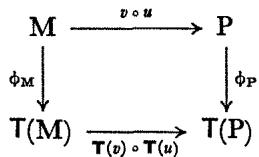
\includegraphics[keepaspectratio]{images/part003_f792dba1.jpg}}

\(\mathsf{T}(u)\) 有时称为 u 到 \(\mathsf{T}(\mathbf{M})\) （它包含 \(\mathbf{M} = \mathsf{T}^1(\mathbf{M})\) ）的典范扩张。注意，限制 \(\mathsf{T}^n(u): \mathsf{T}^n(\mathbf{M}) \to \mathsf{T}^n(\mathbf{N})\) 正是线性映射 \(u^{\otimes n} = u \otimes u \otimes \cdots \otimes u\) （n次），这由下式可知：

\[
\mathsf {T} ^ {n} (u) \left(x _ {1} \otimes \dots \otimes x _ {n}\right) = u \left(x _ {1}\right) \otimes \dots \otimes u \left(x _ {n}\right)
\]

因为 \(\mathsf{T}(u)\) 是一个代数同态且 \(\mathsf{T}^{1}(u)=u\) ；限制 \(\mathsf{T}^{0}(u)\) 在A上是恒等映射。 \(\mathsf{T}^{n}(u)\) 称为u的第n次张量幂。

命题3. 若 \(u: \mathbf{M} \to \mathbf{N}\) 是满射的A-线性映射，则同态 \(\mathsf{T}(u): \mathsf{T}(\mathbf{M}) \to \mathsf{T}(\mathbf{N})\) 是满射的，且其核是 \(\mathsf{T}(\mathbf{M})\) 的由核 \(\mathbf{P} \subset \mathbf{M} \subset \mathsf{T}(\mathbf{M})\) （即 \(u\) 的核）生成的双边理想。

\(T^{0}(u):T^{0}(M)\rightarrow T^{0}(N)\) 是双射的，且对每个整数 n\textgreater0,

\[
\mathbf {T} ^ {n} (u): \mathbf {T} ^ {n} (\mathbf {M}) \rightarrow \mathbf {T} ^ {n} (\mathbf {N})
\]

是满射的，这可通过对 \(n\) 作归纳并利用 II，§ 3，第 6 号，命题 6 看出；后一命题还表明（同样对 \(n\) 作归纳）， \(\mathfrak{S}_n\) （即 \(\mathsf{T}^n(u)\) 的核）是 \(\mathsf{T}^n(\mathbf{M})\) 中由乘积

\[
x _ {1} \otimes x _ {2} \otimes \dots \otimes x _ {n}
\]

生成，其中至少有一个 \(x_{i}\) 属于 \(\mathbf{P}\) 。这表明核 \(\mathfrak{S} = \bigoplus_{n\geqslant 1}\mathfrak{S}_n\) （即 \(\mathsf{T}(u)\) 的核）是由 \(\mathbf{P}\) 在 \(\mathsf{T}(\mathbf{M})\) 中生成的双边理想。

若 \(u: \mathbf{M} \to \mathbf{N}\) 是单射线性映射，则 \(\mathbf{T}(u)\) 并不总是单射映射（练习1）。然而，当 \(u\) 是使 \(u(\mathbf{M})\) 成为 \(\mathbf{N}\) 中直因子的单射时，结论成立，因为此时存在一个线性映射 \(v: \mathbf{N} \to \mathbf{M}\) ，使得 \(v \circ u\) 是 \(\mathbf{M}\) 上的恒等映射，从而

\[
\mathsf {T} (v \circ u) = \mathsf {T} (v) \circ \mathsf {T} (u)
\]

是 \(\mathsf{T}(\mathbf{M})\) 上的恒等映射，因此 \(\mathsf{T}(u)\) 是单射的，且其像（同构于 \(\mathsf{T}(\mathbf{M})\) ）是 \(\mathsf{T}(\mathbf{N})\) 的直因子（II，§1，第9号，命题15）。更精确地说：

命题4. 设N和P是A-模M的两个子模，使得它们的和 \(N + P\) 是M中的直因子，且它们的交 \(N \cap P\) 是N和P中的直因子。则同态 \(\mathsf{T}(\mathbf{N}) \to \mathsf{T}(\mathbf{M})\) , \(\mathsf{T}(\mathbf{P}) \to \mathsf{T}(\mathbf{M})\) 和

\[
\mathsf {T} (\mathbf {N} \cap \mathbf {P}) \rightarrow \mathsf {T} (\mathbf {M}),
\]

典范单射的典范扩张是单射；如果 \(\mathsf{T}(\mathbf{N})\) , \(\mathsf{T}(\mathbf{P})\) 和 \(\mathsf{T}(\mathbf{N} \cap \mathbf{P})\) 通过这些同态被等同于 \(\mathsf{T}(\mathbf{M})\) 的子代数，则

\[
\mathsf {T} (\mathbf {N} \cap \mathbf {P}) = \mathsf {T} (\mathbf {N}) \cap \mathsf {T} (\mathbf {P}).\tag{5}
\]

根据假设，存在子模 \(N' \subset N\) 和 \(P' \subset P\) ，使得 \(N = N' \oplus (N \cap P)\) , \(P = P' \oplus (N \cap P)\) ；于是

\[
\mathbf {N} + \mathbf {P} = \mathbf {N} ^ {\prime} \oplus \mathbf {P} ^ {\prime} \oplus (\mathbf {N} \cap \mathbf {P})
\]

并且根据假设存在子模 \(M'\) ⊂ M，使得

\[
\begin{array}{c} \mathbf {M} = \mathbf {M} ^ {\prime} \oplus (\mathbf {N} + \mathbf {P}) = \mathbf {M} ^ {\prime} \oplus \mathbf {N} ^ {\prime} \oplus \mathbf {P} ^ {\prime} \oplus (\mathbf {N} \cap \mathbf {P}) \\ = \mathbf {M} ^ {\prime} \oplus \mathbf {P} ^ {\prime} \oplus \mathbf {N} = \mathbf {M} ^ {\prime} \oplus \mathbf {N} ^ {\prime} \oplus \mathbf {P}. \end{array}
\]

特别地， \(N + P\) ，N，P以及 \(N \cap P\) 是M中的直因子，这（如前所述）意味着典范同态

\[
\begin{array}{l} \mathsf {T} (\mathbf {N} + \mathbf {P}) \to \mathsf {T} (\mathbf {M}), \qquad \mathsf {T} (\mathbf {N}) \to \mathsf {T} (\mathbf {M}), \\ \mathsf {T} (\mathbf {P}) \to \mathsf {T} (\mathbf {M}), \qquad \mathsf {T} (\mathbf {N} \cap \mathbf {P}) \to \mathsf {T} (\mathbf {M}) \end{array}
\]

是单射的。三个代数 \(\mathsf{T}(\mathbf{N})\) , \(\mathsf{T}(\mathbf{P})\) 和 \(\mathsf{T}(\mathbf{N} \cap \mathbf{P})\) 因此被等同于 \(\mathsf{T}(\mathbf{N} + \mathbf{P})\) 的子代数，而后者被等同于 \(\mathsf{T}(\mathbf{M})\) 的子代数；

记 \(\mathbf{Q} = \mathbf{N} \cap \mathbf{P}\) ，则只需证明：若 \(\mathsf{T}(\mathbf{Q})\) , \(\mathsf{T}(\mathbf{N}' \oplus \mathbf{Q})\) 和 \(\mathsf{T}(\mathbf{P}' \oplus \mathbf{Q})\) 通过这些同态被等同于 \(\mathsf{T}(\mathbf{N}' \oplus \mathbf{P}' \oplus \mathbf{Q})\) 的子代数，则

\[
\mathsf {T} (\mathbf {N} ^ {\prime} \oplus \mathbf {Q}) \cap \mathsf {T} (\mathbf {P} ^ {\prime} \oplus \mathbf {Q}) = \mathsf {T} (\mathbf {Q}).\tag{6}
\]

现在，考虑交换图

\pandocbounded{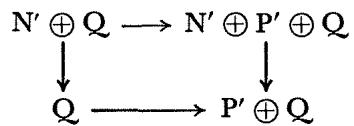
\includegraphics[keepaspectratio]{images/part003_8d12e188.jpg}}

其中水平箭头是典范单射，垂直箭头是典范投影。我们由此导出一个交换图

\begin{enumerate}
\def\labelenumi{(\arabic{enumi})}
\setcounter{enumi}{6}
\tightlist
\item
\end{enumerate}

\pandocbounded{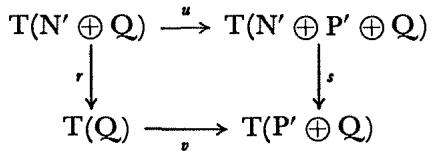
\includegraphics[keepaspectratio]{images/part003_389443db.jpg}}

其中 r 和 s 是满同态（命题 3），而 u 和 v 是单同态。因此，为证明 (6)，注意到右端显然包含于左端；于是只需验证：若

\[
x \in \mathsf {T} (\mathbf {N} ^ {\prime} \oplus \mathbf {Q}) \cap \mathsf {T} (\mathbf {P} ^ {\prime} \oplus \mathbf {Q}),
\]

那么 \(x \in \mathsf{T}(\mathsf{Q})\) 。现在，同态 s 的定义表明，它在 \(\mathsf{T}(\mathsf{P}' \oplus \mathsf{Q})\) （等同于 \(\mathsf{T}(\mathsf{N}' \oplus \mathsf{P}' \oplus \mathsf{Q})\) 的一个子代数）上的限制是恒等映射；因此关于 x 的假设蕴含 \(s(u(x)) = x\) 。但此时也有 \(v(r(x)) = x\) ，换言之，x 属于 \(\mathsf{T}(\mathsf{Q})\) 在 \(\mathsf{T}(\mathsf{P}' \oplus \mathsf{Q})\) 中的像，这就是要证明的。

注。特别地，当 A 是域时（II，§ 7，第 3 号，命题 4），命题 4 的假设对 M 的任意子模 N, P 总是成立。此外，若 N ⊂ P 且 N ≠ P，则对所有 n ≥ 1 有 T \(^{n}\) (N) ≠ T \(^{n}\) (P)，因为如果 R 是 P 在 N 中的补，则 T \(^{n}\) (P) ∩ T \(^{n}\) (R) = \{0\} 由(4)及T \(^{n}\) (R) ≠ \{0\}.

推论。设K是一个交换域，M是K上的一个向量空间。对于每一个元素 \(z \in \mathsf{T}(\mathbf{M})\) 存在一个M的最小子空间N，使得 \(z \in \mathsf{T}(\mathbf{N})\) 且N在K上具有有限秩。

在这个陈述中约定，对于 M 的每个向量子空间 P， \(T(P)\) 典范地等同于 \(T(M)\) 的一个子代数。设 \(z \in T(M)\) ；z 可以表示为一些元素的线性组合，其中每个元素都是 \(M = T^{1}(M)\) 中元素的有限乘积；出现在这些乘积中的 M 的所有元素生成一个有限秩的向量子空间 Q，且 \(z \in T(Q)\) .

设 \(\mathfrak{F}\) 为由有限秩向量子空间 \(\mathbf{P}\) （满足 \(z\in \mathsf{T}(\mathbf{P})\) ）组成的（非空）集合。 \(\mathfrak{F}\) 中元素的每个递减序列都是平稳的，因为它们是有限秩的向量空间。因此 \(\mathfrak{F}\) 有一个极小元素 \(\mathbf{N}\) （集合论，III，§6，第5号）。还需验证每个 \(\mathbf{P}\in \mathfrak{F}\) 包含 \(\mathbf{N}\) ；现在， \(z\in \mathsf{T}(\mathbf{P})\cap \mathsf{T}(\mathbf{N}) = \mathsf{T}(\mathbf{P}\cap \mathbf{N})\) （命题4）；根据 \(\mathbf{N}\) 的定义，这意味着 \(\mathbf{N}\cap \mathbf{P} = \mathbf{N}\) ，即 \(\mathbf{P}\supset \mathbf{N}\) .

M的子空间N称为与z相关联的。

